% !TEX root = main.tex
\begin{figure}[t]
\vspace{-0.9cm}
\center
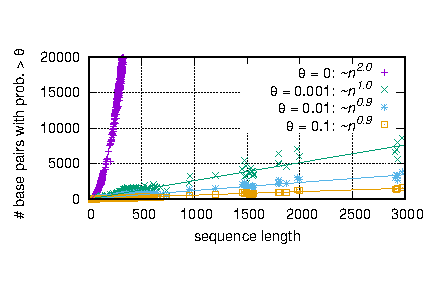
\includegraphics[width=.42\textwidth]{figs/Vienna_RNAfold_num_pij_curves.pdf}\\[-1cm]
\caption{
  Although the total number of possible base pairings scales $O(n^2)$ with the sequence length $n$
  (using the probability matrix from \viennarnafold as an example),
  with any reasonable threshold $\theta$, the number of surviving pairings (in colors for different $\theta$) grows linearly,
  suggesting our approximation, only computing $O(n)$ pairings, is reasonable.
  \label{fig:linearpairs}}
\vspace{-0.7cm}
\end{figure}
